\vspace{\sectionSpace}
\section{Experiments}
\label{sec:experiments}

\begin{figure*}[!ht]
\subfloat[local]{
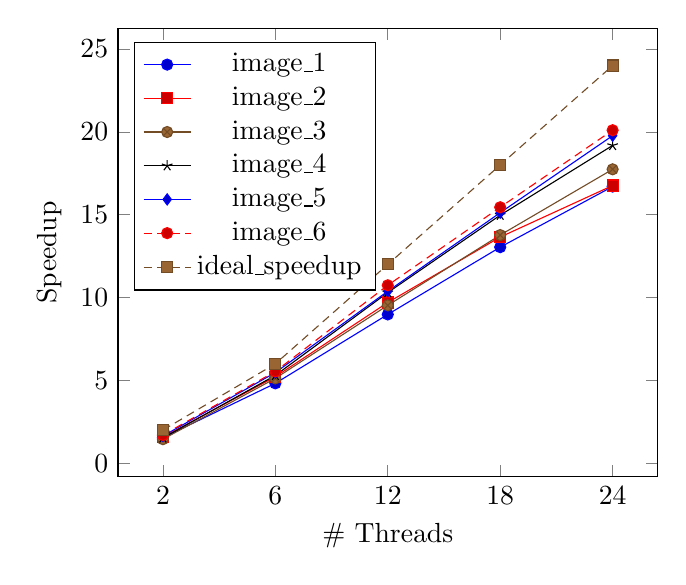
\begin{tikzpicture}
\begin{axis}[legend pos = north west,
xlabel=\# Threads,
ylabel=Speedup,
symbolic x coords={2,6,12,18,24}]

\addplot+[sharp plot] coordinates{
(2,1.54)
(6,4.82)
(12,8.98)
(18,13.04)
(24,16.70)
};
\addplot+[sharp plot] coordinates {
(2,1.58)
(6,5.22)
(12,9.7)
(18,13.65)
(24,16.76)
};
\addplot+[sharp plot] coordinates{
(2,1.45)
(6,5.12)
(12,9.53)
(18,13.77)
(24,17.74)
};
\addplot+[sharp plot] coordinates{
(2,1.53)
(6,5.30)
(12,10.30)
(18,14.97)
(24,19.18)
};
\addplot+[sharp plot] coordinates{
(2,1.64)
(6,5.47)
(12,10.38)
(18,15.12)
(24,19.77)
};

\addplot+[sharp plot] coordinates{
(2,1.7)
(6,5.54)
(12,10.74)
(18,15.45)
(24,20.10)
};
\addplot+[sharp plot] coordinates{
(2,2)
(6,6)
(12,12)
(18,18)
(24,24)
};
\legend{image\_1,image\_2,image\_3,image\_4,image\_5,image\_6,ideal\_speedup}
\end{axis}
\end{tikzpicture}
\label{line}
}
\subfloat[local + merge]{
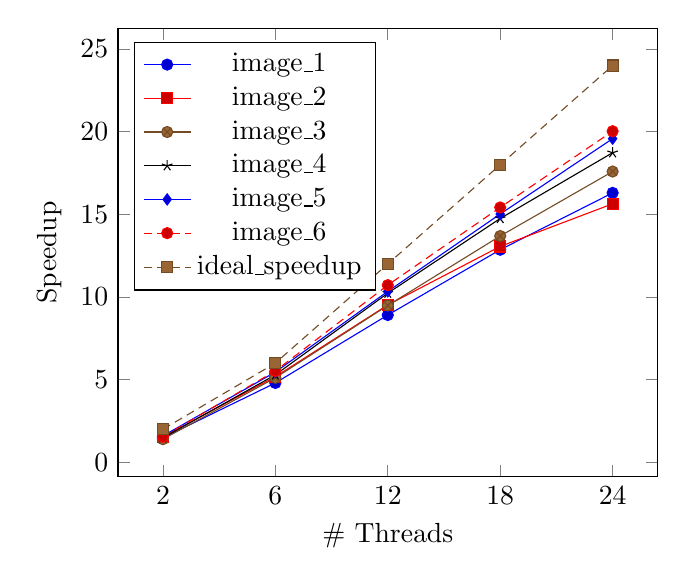
\begin{tikzpicture}
\begin{axis}[legend pos = north west,
xlabel=\# Threads,
ylabel=Speedup,
symbolic x coords={2,6,12,18,24}]
\addplot+[sharp plot] coordinates{
(2,1.48)
(6,4.80)
(12,8.91)
(18,12.86)
(24,16.30)
};

\addplot+[sharp plot] coordinates {
(2,1.54)
(6,5.18)
(12,9.52)
(18,13.06)
(24,15.64)
};
\addplot+[sharp plot] coordinates{
(2,1.40)
(6,5.11)
(12,9.49)
(18,13.69)
(24,17.59)
};

\addplot+[sharp plot] coordinates{
(2,1.49)
(6,5.29)
(12,10.23)
(18,14.75)
(24,18.73)
};

\addplot+[sharp plot] coordinates{
(2,1.60)
(6,5.46)
(12,10.34)
(18,15.02)
(24,19.58)
};


\addplot+[sharp plot] coordinates{
(2,1.55)
(6,5.53)
(12,10.72)
(18,15.42)
(24,20.03)
};
\addplot+[sharp plot] coordinates{
(2,2)
(6,6)
(12,12)
(18,18)
(24,24)
};
\legend{image\_1,image\_2,image\_3,image\_4,image\_5,image\_6,ideal\_speedup}
\end{axis}
\end{tikzpicture}
% \caption{Speedup for different images and different numbers of threads for local + merge}
\label{linet}
}
\caption{Speedup for different images and different numbers of threads for NLCD
dataset}
\label{speed}
\end{figure*}


For the experiments we used a computing node of Hopper, a Cray XE6 distributed memory parallel computer. 
The node has 2 twelve-core AMD ‘MagnyCours’ 2.1-GHz processors and 32 GB DDR3 1333-MHz memory. 
Each core has its own L1 and L2 caches, with 64 KB and 512 KB, respectively. 
One 6-MB L3 cache is shared between 6 cores on the MagnyCours processor. 
All algorithms were implemented in C using OpenMP and compiled with gcc.

Our test data set consists of four types of image data set: Texture, Aerial,
Miscellaneous and NLCD. First three data sets are taken from the image database of the University of 
Southern
California.\footnote{\url{http://sipi.usc.edu/database/}} 
The fourth data set is taken from US National Cover Database
$2006$.\footnote{\url{http://dx.doi.org/10.1016/j.cageo.2013.05.014}} All of the
images are converted to binary images by MATLAB using $im2bw(level)$ function with level value as $0.5$. The function 
converts the grayscale image to a binary image by replacing all pixels in the input image with luminance greater than 
0.5 with the value 1 (white) and replaces all other pixels with the value 0 (black). If the input image is not a grayscale image, 
$im2bw$ converts the input image to grayscale, and then converts this grayscale image to binary. However, note that our
algorithm can be easily extended to gray scale images.

Texture, Aerial and Miscellaneous data set contain images of size $1$ MB or less.
NCLD data set contains images of size bigger than $12$ MB. The biggest image in the data set is $465.20$ MB.

Firstly, we performed the experiment over all the sequential algorithms. The
experimental results are shown in Table \ref{table:seq}. In the table, we have
shown the minimum, maximum and average execution time of all the four data sets. 
\begin{algorithm}[ht!]
\small
{
	\caption{Pseudo-code for ARemSP Scan Phase}
	\label{alg:ARemSP-I}
	\textbf{Input:} $2D$ array $image$ containing the pixel values \\
	\textbf{InOut:} $2D$ array $label$ containing the provisional labels and $1D$ array $p$ containing the equivalence info\\
	\textbf{Output:} maximum value of
	provisional label in $count$
	\begin{algorithmic}[1]
	\Function{Scan\_ARemSP}{$image$}
		\For{$row$ in $image$}
			\For{$col$ in $row$}
				\If{$image(e) = 1$}
					\If{$image(d) = 0$}
						\If{$image(b) = 1$}
							\State $label(e) \gets label(b)$
							\If{$image(f) = 1$}
								\State $merge(p,label(e),label(f))$ 
							\EndIf
						\Else
							\If{$image(f) = 1$}
								\State $label(e) \gets label(f)$
								\If{$image(a) = 1$}
									\State $merge(p,label(a))$
								\EndIf
								\If{$image(c) = 1$}
									\State $merge(p,label(e),label(c))$
								\EndIf
							\Else
								\If{$image(a) = 1$}
									\State $label(e) \gets label(a)$
									\If{$image(c) = 1$}
										\State $merge(p,label(e),label(c))$
									\EndIf
								\Else
									\If{$image(c) = 1$}
										\State $label(e) \gets label(c)$
									\Else
										\State $label(e) \gets count,$
										\State $p[count] \gets count,$
										\State $count++$
									\EndIf
								\EndIf
							\EndIf
						\EndIf
					\Else
						\State $label(e) = label(d)$
						\If{$image(b) = 0$}
							\If{$image(c) = 1$}
								\State $merge(p,label(e),label(c))$
							\EndIf
						\EndIf
					\EndIf
					\If{$image(g) = 1$}
						\State $label(g) \gets label(e)$
					\EndIf
				\Else
					\If{$image(g) = 1$}
						\If{$image(d) = 1$}
							\State $label(g) \gets label(d)$
						\Else
							\If{$image(f) = 1$}
								\State $label(g) \gets label(f)$
							\Else
								\State $label(e) \gets count,$
								\State $p[count] \gets count,$
								\State $count++$
							\EndIf
						\EndIf
					\EndIf
				\EndIf
			\EndFor
		\EndFor
		\State \Return {$count$}
	\EndFunction
	\end{algorithmic}	
}
\end{algorithm}


\begin{table}[h!]
\caption{Comparison of various execution times[{\em msec}] for sequential algorithms}
\centering
\begin{tabular}{c c c c c c} 
\hline\hline
Image type &  & CCLLRPC & CCLRemSP & ARun & ARemSP\\ [0.25ex] 
\hline 
Aerial & Min & 2.5 & 2.48 & 1.98 & 1.95 \\ 
 & Average & 13.68 & 13.25 & 11.90 & 11.86\\
 & Max & 86.64 & 80.90 & 72.92 & 70.17 \\
[0.25ex]
 \hline
Texture & Min &2.07 & 2.06 & 1.58 & 1.53 \\
 & Average & 8.42 & 8.20 & 7.32 & 7.27 \\
 & Max & 16.86 & 16.18 & 14.81 & 14.47\\
[0.25ex]
 \hline
Misc & Min & 0.50 & 0.49 & 0.36 & 0.36\\
 & Average & 3.28 & 3.21 & 2.75 & 2.74 \\
 & Max &12.96 & 12.81 & 11.30 & 11.20\\
 [0.25ex]
\hline
NLCD & Min & 4.61 & 4.46	& 3.77 & 3.75 \\
& Average & 307.66 & 299.55 & 244.88 & 242.59 \\
& Max & 1307.27	& 1273.82 & 1036.52 & 1021.45
\\[0.25ex]
\hline
\end{tabular}
\label{table:seq} 
\end{table}

\begin{table}[h]
\caption{Images and their sizes [in {\em MB}]}
\centering
\begin{tabular}{c c} 
\hline\hline
Image name & Size\\ [0.5ex] 
\hline 
image\_1 & $12$\\
image\_2 & $33$ \\
image\_3 & $37.31$ \\
image\_4 & $116.30$ \\
image\_5 & $132.03$\\ 
image\_6 & $465.20$\\
[1ex]
\hline
\end{tabular}
\label{table:imag_size} 
\end{table}

\begin{table}[h]
\caption{Execution time [{\em msec}] of \paremsp\ algorithm for various \#
threads}
\centering
\begin{tabular}{c c c c c c} 
\hline\hline
Image type &  & 2 & 6 & 16 & 24\\ [0.5ex] 
\hline 
Aerial & Min & 1.39 & 0.84 & 1.02 & 1.38 \\ 
 & Average & 7.92	& 3.03	& 1.87	& 2.15
\\
 & Max & 46.86 &	16.72 & 	7.32 &	6.97
 \\
[1ex]
 \hline
Texture & Min & 1.09 & 0.62 & 	0.93 &	1.36
 \\
 & Average & 4.91 &	1.99 &	1.45	& 1.82
 \\
 & Max & 9.75 &	3.56 &	2.11 &	2.34
\\
[1ex]
 \hline
Miscellaneous & Min & 0.36	& 0.36	& 0.79	& 1.18
\\
 & Average & 1.99	& 0.97	& 1.05	& 1.46
 \\
 & Max &7.96	& 3.24	& 1.91	& 2.27
\\
 [1ex]
\hline
NLCD & Min & 2.52& 1.16&	1.32&	1.67
\\
& Average & 162.86&	58.50&	20.20&	13.47
 \\
& Max & 676.41	&184.71	&78.33	&51.00
 \\[1ex]
\hline
\end{tabular}
\label{table:seq} 
\end{table}


As we can see that execution time of \aremsp\ is lowest among all
the sequential algorithms. Thus \aremsp\ is best among all the sequential
algorithms.
Next, we show our results for the parallel algorithm \paremsp\ over all the images.
Figure \ref{line}-\ref{linet} show the speedup of the algorithm for 
NCLD image data set. The size of the images are given in Table \ref{table:sequ}.
We get a maximum speedup of $20.1$ on $24$ cores for image of size $465.20$ MB.

Figure \ref{line} shows the speedup for {\em Phase-$I$} of \paremsp\ i.e. 
the local computation and Figure \ref{linet} shows the overall speedup (i.e.
local + merge). We can see that there is not significant difference between both speedups, implying that merge operation
does not have a significant overhead. 
Also as can be seen from the graph, as the image size increases, speedup also
increases. Therefore, our parallel implementation is able to achieve near linear
speed for large data sets. We have also shown the speedup for all the other data sets in Figure \ref{bar}.
The minimum, maximum and average execution time of \paremsp\ for all the datasets is also shown in Table \ref{table:par}.
We get a maximum speedup of $10$ in this case as the images are $1$ MB or less in size. The speedup also decreases in some cases as the
number of threads increases.
This is because the image size is small so as the number of threads increases,
the threads will have less work to perform and the overhead due to thread
creation will increase.
\begin{figure}
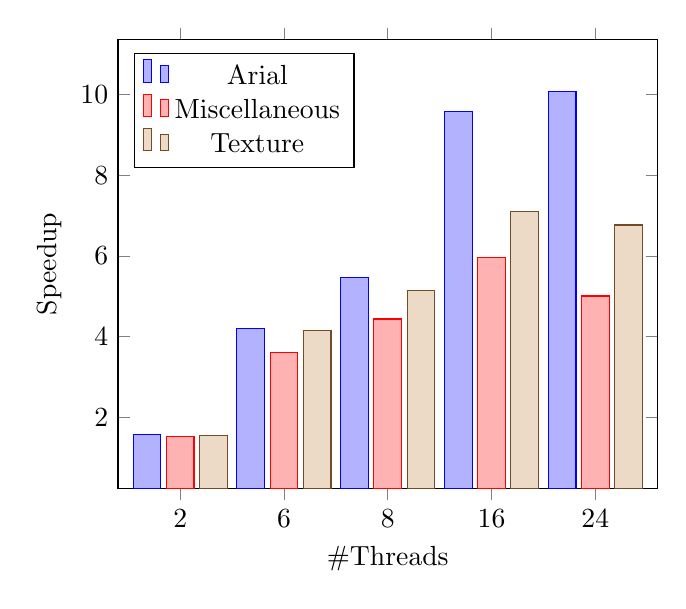
\begin{tikzpicture}
\begin{axis}[
ybar,
enlargelimits=0.15,
legend pos = north west,
xlabel=\#Threads,
ylabel=Speedup,
symbolic x coords={2,6,8,16,24},
xtick=data,
]
\addplot
coordinates {
(2,1.57)
(6,4.20)
(8,5.46)
(16,9.58)
(24,10.08)

};
\addplot
coordinates {
(2,1.53)
(6,3.60)
(8,4.44)
(16,5.96)
(24,5.01)
};
\addplot
coordinates {
(2,1.56)
(6,4.16)
(8,5.14)
(16,7.10)
(24,6.77)
};

\legend{Arial,Miscellaneous,Texture}
\end{axis}
\end{tikzpicture}
\caption{Speedup for different images and different numbers of threads}
\label{bar}
\end{figure}


